\section{Snake}

\begin{figure}[htbp]
\begin{center}
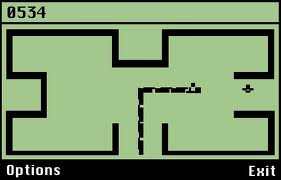
\includegraphics[width=.60\textwidth]{./imagenes/snake.png}
\caption{Snake}
\label{Snake}
\end{center}
\end{figure}
Snake\footnote{\url{http://www.snakegame.net/}} en este juego, el jugador controla una larga y delgada criatura, semejante a una serpiente, que vaga alrededor de un plano delimitado, recogiendo alimentos (o algún otro elemento), tratando de evitar golpear a su propia cola o las "paredes" que rodean el área de juego. Cada vez que la serpiente se come un pedazo de comida, la cola crece más, provocando que aumente la dificultad del juego. El usuario controla la dirección de la cabeza de la serpiente (arriba, abajo, izquierda o derecha) y el cuerpo de la serpiente la sigue. Además, el jugador no puede detener el movimiento de la serpiente, mientras que el juego está en marcha.

\subsubsection{¿Por qué es uno de mis juegos favoritos?}
\begin{itemize}
\item Es uno de mis juegos favoritos porque mientras que la serpiente va comiendo, esta crece y la dificultad del juego aumentan, porque queda menos espacio para que la serpiente siga transitando.
Y además el juego cuenta con algunas variantes, que puede hacer que el juego aumente la dificultad y hacer más interesante el juego.

\end{itemize}
